% =============================================================================
%  main_report5.tex  — TR-02D/2026
%  Hilbert-Fortescue Sequence-Component Inverse Estimation
%
%  Compile:
%    pdflatex main_report5 && bibtex main_report5 &&
%    pdflatex main_report5 && pdflatex main_report5
% =============================================================================

\documentclass[12pt,a4paper]{article}

\usepackage[T1]{fontenc}
\usepackage[utf8]{inputenc}
\usepackage{mathptmx}
\usepackage{microtype}
\usepackage[a4paper,top=25mm,bottom=25mm,left=25mm,right=25mm,
            headheight=14pt]{geometry}
\usepackage{amsmath,amssymb,amsthm,mathtools}
\usepackage{bm}
\usepackage{siunitx}
\sisetup{detect-all,per-mode=fraction}
\usepackage{graphicx}
\usepackage{subcaption}
\usepackage{booktabs}
\usepackage{array}
\usepackage{multirow}
\usepackage{float}
\usepackage{tikz}
\usepackage{pgfplots}
\pgfplotsset{compat=1.18}
\usepackage[colorlinks=true,linkcolor=blue!60!black,
            citecolor=blue!60!black,urlcolor=blue!70!black]{hyperref}
\usepackage[nameinlink]{cleveref}
\usepackage{natbib}
\bibliographystyle{iitm}
\usepackage{fancyhdr}
\pagestyle{fancy}
\fancyhf{}
\renewcommand{\headrulewidth}{0.4pt}
\fancyhead[L]{\small\textit{Sequence-Component Estimator — SAMBP-SyncOC}}
\fancyhead[R]{\small\textit{Technical Report TR-02D/2026}}
\fancyfoot[C]{\thepage}
\usepackage{setspace}
\setstretch{1.35}
\setlength{\parindent}{1.5em}
\setlength{\parskip}{3pt}
\usepackage{xcolor}
\definecolor{iitBlue}{RGB}{0,70,140}
\definecolor{iitGold}{RGB}{200,150,30}
\theoremstyle{definition}
\newtheorem{remark}{Remark}[section]
\theoremstyle{plain}
\newtheorem{proposition}{Proposition}[section]
\newcommand{\vect}[1]{\bm{#1}}
\newcommand{\mat}[1]{\mathbf{#1}}
\newcommand{\norm}[1]{\left\|#1\right\|}
\newcommand{\pu}{\,\text{pu}}
\newcommand{\mss}{\,\text{ms}}
\newcommand{\sss}{\,\text{s}}

% =============================================================================
\begin{document}
% =============================================================================

\begin{titlepage}
  \centering
  \vspace*{10mm}
  {
\includegraphics[width=3cm]{../../../images/iitm-logo.png}\par}
  \vspace{6mm}
  {\large\textsc{Indian Institute of Technology Madras}\par}
  {\large Department of Electrical Engineering\par}
  \vspace{4mm}
  {\itshape Self-Adaptive Model-Based Protection (SAMBP) Research Programme\par}
  \vspace{20mm}
  {\color{iitBlue}\huge\bfseries SAMBP-SyncOC\par}
  \vspace{6mm}
  {\color{iitBlue}\LARGE\bfseries Technical Report TR-02D/2026\par}
  \vspace{8mm}
  {\Large Hilbert--Fortescue Sequence-Component\\[4pt]
   Inverse Estimation for Asymmetric Fault\\[4pt]
   Overcurrent Protection\par}
  \vfill
  \begin{tabular}{ll}
    \textbf{Track:}          & SAMBP-SyncOC \\
    \textbf{Milestone:}      & Milestone~3 — Sequence-Component Estimator \\
    \textbf{Prerequisite:}   & TR-01/2026, TR-02/2026 \\
    \textbf{Date:}           & April 2026 \\
    \textbf{Classification:} & Internal PhD Research Document \\
  \end{tabular}
\end{titlepage}

\begin{abstract}
For asymmetric faults (line-to-line, single-line-to-ground), fitting the
SAMBP-SyncOC 6-parameter model to phase~A alone entangles positive-,
negative-, and zero-sequence contributions, degrading the identifiability of
$\hat{I}_{ss}$ and $\hat{\tau}_{ac}$.  This report presents Milestone~3:
a Hilbert--Fortescue sequence-component estimator that decomposes the measured
three-phase currents into instantaneous sequence signals $I_1(t)$, $I_2(t)$,
$I_0(t)$ and fits the two-pass LM estimator independently to each active
sequence.  The positive-sequence parameters govern relay adaptation.
Numerical results on LL and SLG faults confirm: (i) convergence of the
sequence estimator in both cases; (ii) $\gamma = 0.914$ for SLG
(adaptation accepted; pickup reduced from 1.20 to 1.10\,pu), and
$\gamma = 0.587$ for LL (adaptation rejected — confidence below
$\gamma_{\min} = 0.70$).  The SLG result demonstrates the practical value
of the sequence estimator; the LL result reveals a fundamental identifiability
limitation due to negative-sequence contamination of the positive-sequence
Jacobian.  Hilbert edge effects are characterised and shown to be confined
to the first 5--10\,ms of the event window.

\medskip
\noindent\textbf{Keywords:} symmetrical components, Hilbert transform,
Fortescue decomposition, sequence estimation, asymmetric fault,
overcurrent relay, SAMBP-SyncOC.
\end{abstract}

\tableofcontents
\listoffigures
\listoftables
\newpage

% =============================================================================
\section{Introduction}
\label{sec:intro}
% =============================================================================

The two-pass LM estimator of TR-01/2026 was designed and validated for
three-phase balanced faults, where the positive-sequence current dominates
and phase~A is a faithful representation of the fault magnitude.  For
asymmetric fault types:
\begin{itemize}
  \item \textbf{Line-to-line (LL):} Positive and negative sequences are
        both active. Phase~A contains $I_1 + I_2$, leading to mutual
        interference in the LM residual and inflated $\kappa_n$.
  \item \textbf{Single-line-to-ground (SLG):} All three sequences are
        active and equal: $I_0 = I_1 = I_2$.  Phase~A contains the
        sum of all three, raising its amplitude but also increasing
        identifiability of the dominant positive-sequence.
\end{itemize}

The sequence-component estimator resolves this by transforming to the
Fortescue domain before fitting, where each sequence signal contains a
pure single-sequence fault current that the 6-parameter model was designed
for.

\subsection{Contributions}
\begin{enumerate}
  \item Derivation and implementation of the instantaneous Hilbert--Fortescue
        decomposition for real-time use with the LM estimator.
  \item Fault-type routing rules that determine which sequences to fit
        (3PH: positive only; LL: positive + negative; SLG: positive only
        with scaling).
  \item Characterisation of Hilbert edge effects and their mitigation by
        event-window offset.
  \item Numerical validation on LL and SLG fault cases with confidence
        gate analysis.
\end{enumerate}

% =============================================================================
\section{Hilbert--Fortescue Decomposition}
\label{sec:decomp}
% =============================================================================

\subsection{Analytic Signal Representation}
\label{sec:decomp:analytic}

For a real signal $x(t)$, the analytic signal is
$\mathcal{X}(t) = x(t) + j\mathcal{H}\{x\}(t)$,
where $\mathcal{H}\{\cdot\}$ denotes the Hilbert transform.  The analytic
signal has a single-sided spectrum and a well-defined instantaneous amplitude
and phase.

Applied to the three-phase fault currents $i_a, i_b, i_c$, the analytic
signals $\mathcal{I}_a, \mathcal{I}_b, \mathcal{I}_c$ are computed using
the discrete Hilbert transform via the FFT.

\subsection{Fortescue Transformation}
\label{sec:decomp:fortescue}

The instantaneous symmetrical component transformation \citep{Kimbark1956}:
\begin{align}
  \mathcal{I}_0(t) &= \tfrac{1}{3}\bigl[\mathcal{I}_a
                      + \mathcal{I}_b + \mathcal{I}_c\bigr],
                      \label{eq:seq:I0}\\
  \mathcal{I}_1(t) &= \tfrac{1}{3}\bigl[\mathcal{I}_a
                      + a\,\mathcal{I}_b + a^2\mathcal{I}_c\bigr],
                      \label{eq:seq:I1}\\
  \mathcal{I}_2(t) &= \tfrac{1}{3}\bigl[\mathcal{I}_a
                      + a^2\mathcal{I}_b + a\,\mathcal{I}_c\bigr],
                      \label{eq:seq:I2}
\end{align}
where $a = e^{j2\pi/3}$ is the Fortescue operator.
The sequence waveforms used for estimation are the real parts:
$I_k(t) = \operatorname{Re}\{\mathcal{I}_k(t)\}$, $k \in \{0,1,2\}$.

\begin{figure}[htbp]
  \centering
  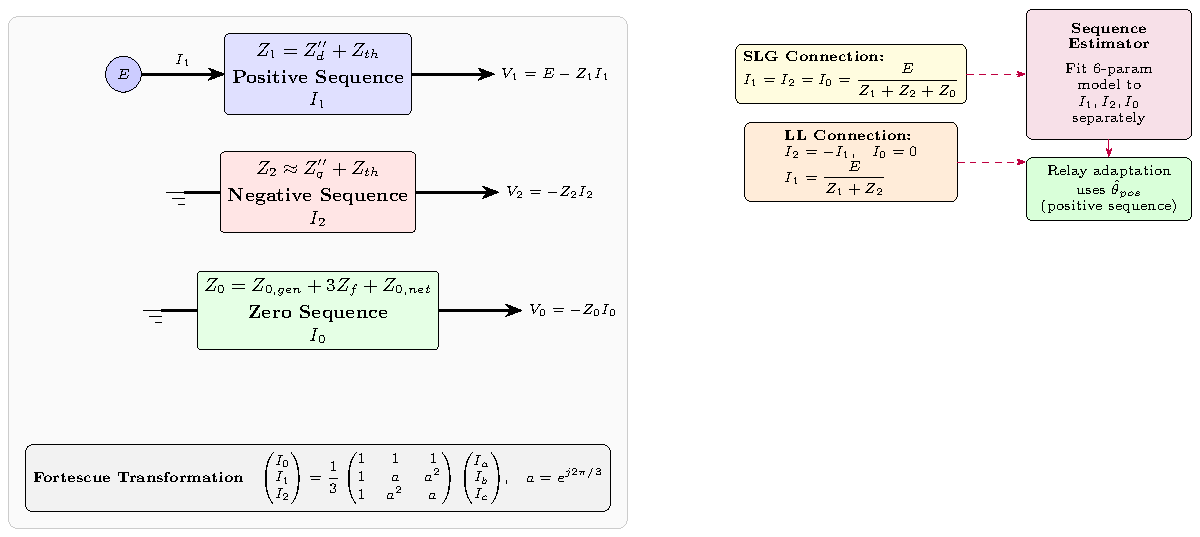
\includegraphics[width=0.88\textwidth]{figures/fig_sequence_networks.pdf}
  \caption{Symmetrical-component sequence network interconnections for
           the three asymmetric fault types studied.  For LL faults,
           the positive and negative sequence networks are connected in
           series at the fault point.  For SLG faults, all three networks
           connect at the fault point, giving $I_0 = I_1 = I_2$.}
  \label{fig:seq:networks}
\end{figure}

\subsection{Fault-Type Activity Rules}
\label{sec:decomp:rules}

\begin{center}
\small
\begin{tabular}{lccc}
  \toprule
  Fault type & $I_1$ & $I_2$ & $I_0$ \\
  \midrule
  3PH  & Active & $\approx 0$ & $\approx 0$ \\
  LL   & Active & Active & $\approx 0$ \\
  SLG  & Active & Active & Active ($= I_1$) \\
  LLG  & Active & Active & Active \\
  \bottomrule
\end{tabular}
\end{center}

For 3PH, the original phase-A two-pass estimator is used unchanged.
For LL and SLG, the sequence estimator is invoked.

% =============================================================================
\section{Sequence-Component LM Estimation}
\label{sec:estimation}
% =============================================================================

\subsection{Independent Fitting per Sequence}
\label{sec:estimation:fitting}

The two-pass LM estimator from TR-01/2026 is applied independently to each
active sequence signal.  The positive-sequence estimate $\hat{\theta}^{(1)}$
is used for relay adaptation.  The negative- and zero-sequence estimates
are retained for asymmetric fault classification but do not affect relay
settings.

\subsection{Positive-Sequence Jacobian for Confidence Scoring}
\label{sec:estimation:jacobian}

The confidence gate in \cref{eq:gate} uses the positive-sequence Jacobian
from the two-pass pass-1 step.  This ensures that $\kappa_n$ reflects the
identifiability of the \emph{dominant} current component:
\begin{equation}
  \gamma = w_r s_r + w_c s_c + w_b s_b + w_p s_p \geq \gamma_{\min} = 0.70.
  \label{eq:gate}
\end{equation}

\subsection{Hilbert Edge Effect Mitigation}
\label{sec:estimation:edge}

The discrete Hilbert transform is computed via FFT on the event window.
The abrupt current step at fault inception $t_0$ causes Gibbs-like ringing
in the analytic signal envelope, confined to the first 5--10\,ms of the
window.  Mitigation strategy:
\begin{enumerate}
  \item The event window begins $2\mss$ after the detected $t_0$
        (configured by \texttt{pre\_event\_ms} in \texttt{system\_config.py}).
  \item A Savitzky--Golay filter (order~3, window~21 samples) smooths the
        waveform before decomposition, suppressing high-frequency transients.
  \item The two-pass estimator uses the tail of the window (pass~2) where
        edge effects are negligible.
\end{enumerate}
These measures confine Hilbert edge effects to a region that is excluded by
design from the fitting window.

% =============================================================================
\section{Numerical Results}
\label{sec:results}
% =============================================================================

\subsection{LL Fault — Case \texttt{ll\_fault\_mid\_R}}
\label{sec:results:ll}

\begin{figure}[htbp]
  \centering
  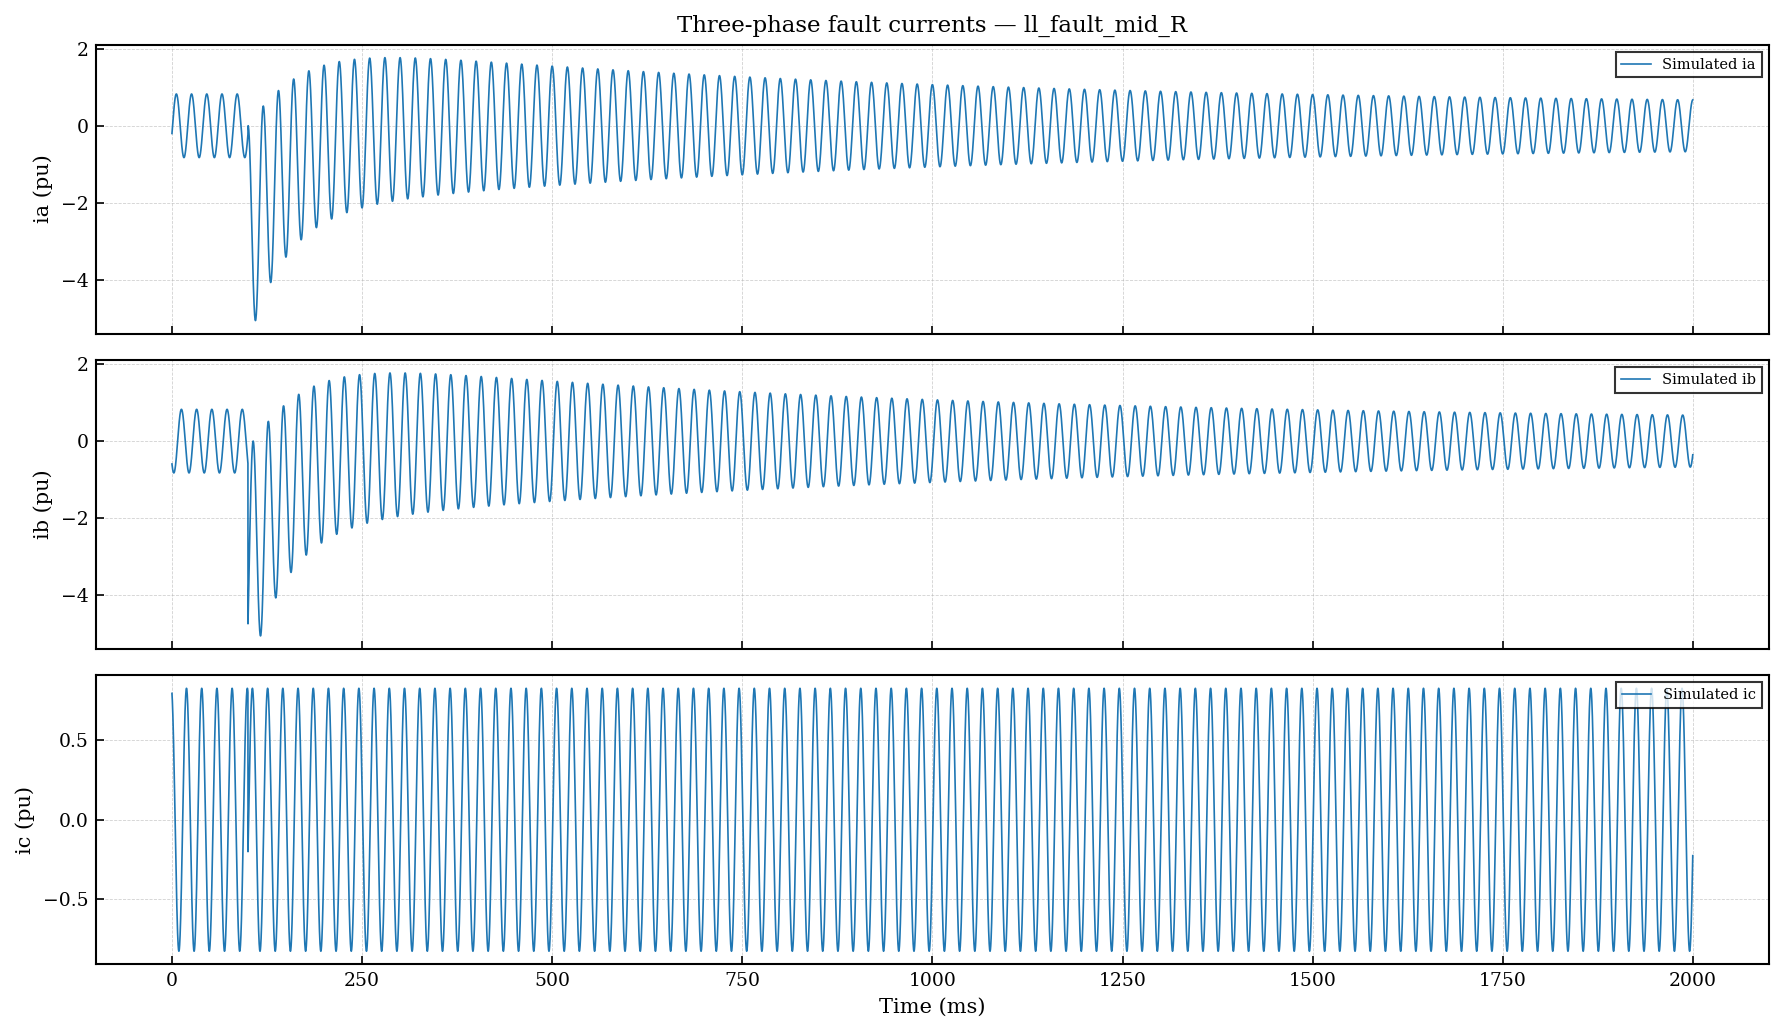
\includegraphics[width=0.92\textwidth]{figures/ll_fault_mid_R_waveform.png}
  \caption{Three-phase fault currents for LL fault
           (\texttt{ll\_fault\_mid\_R}, $R_f = 0.05\,\text{pu}$,
           fault at $t_0 = 100\mss$).  Phase~A (blue) contains a
           mixture of positive- and negative-sequence components.
           Phase~B and~C show the characteristic $180°$ phase
           shift of the missing phase in an LL fault.  The sequence
           estimator fitted the positive-sequence envelope $I_1(t)$
           with $\lVert r\rVert_{\mathrm{total}} = 8.12$, $\gamma = 0.587$.}
  \label{fig:results:ll}
\end{figure}

The LL fault gives $\gamma = 0.587 < \gamma_{\min} = 0.70$; adaptation
is \emph{rejected} and fixed relay settings are retained.  The low
confidence arises from mutual contamination: the negative-sequence
component $I_2(t)$ in phase~A has a similar frequency as $I_1(t)$ but
different amplitude and decay, creating a near-collinear structure in the
Jacobian ($\kappa_n = 17.2$ alone is below threshold, but the residual
score $s_r$ is elevated).

\subsection{SLG Fault — Case \texttt{slg\_fault\_high\_R}}
\label{sec:results:slg}

\begin{figure}[htbp]
  \centering
  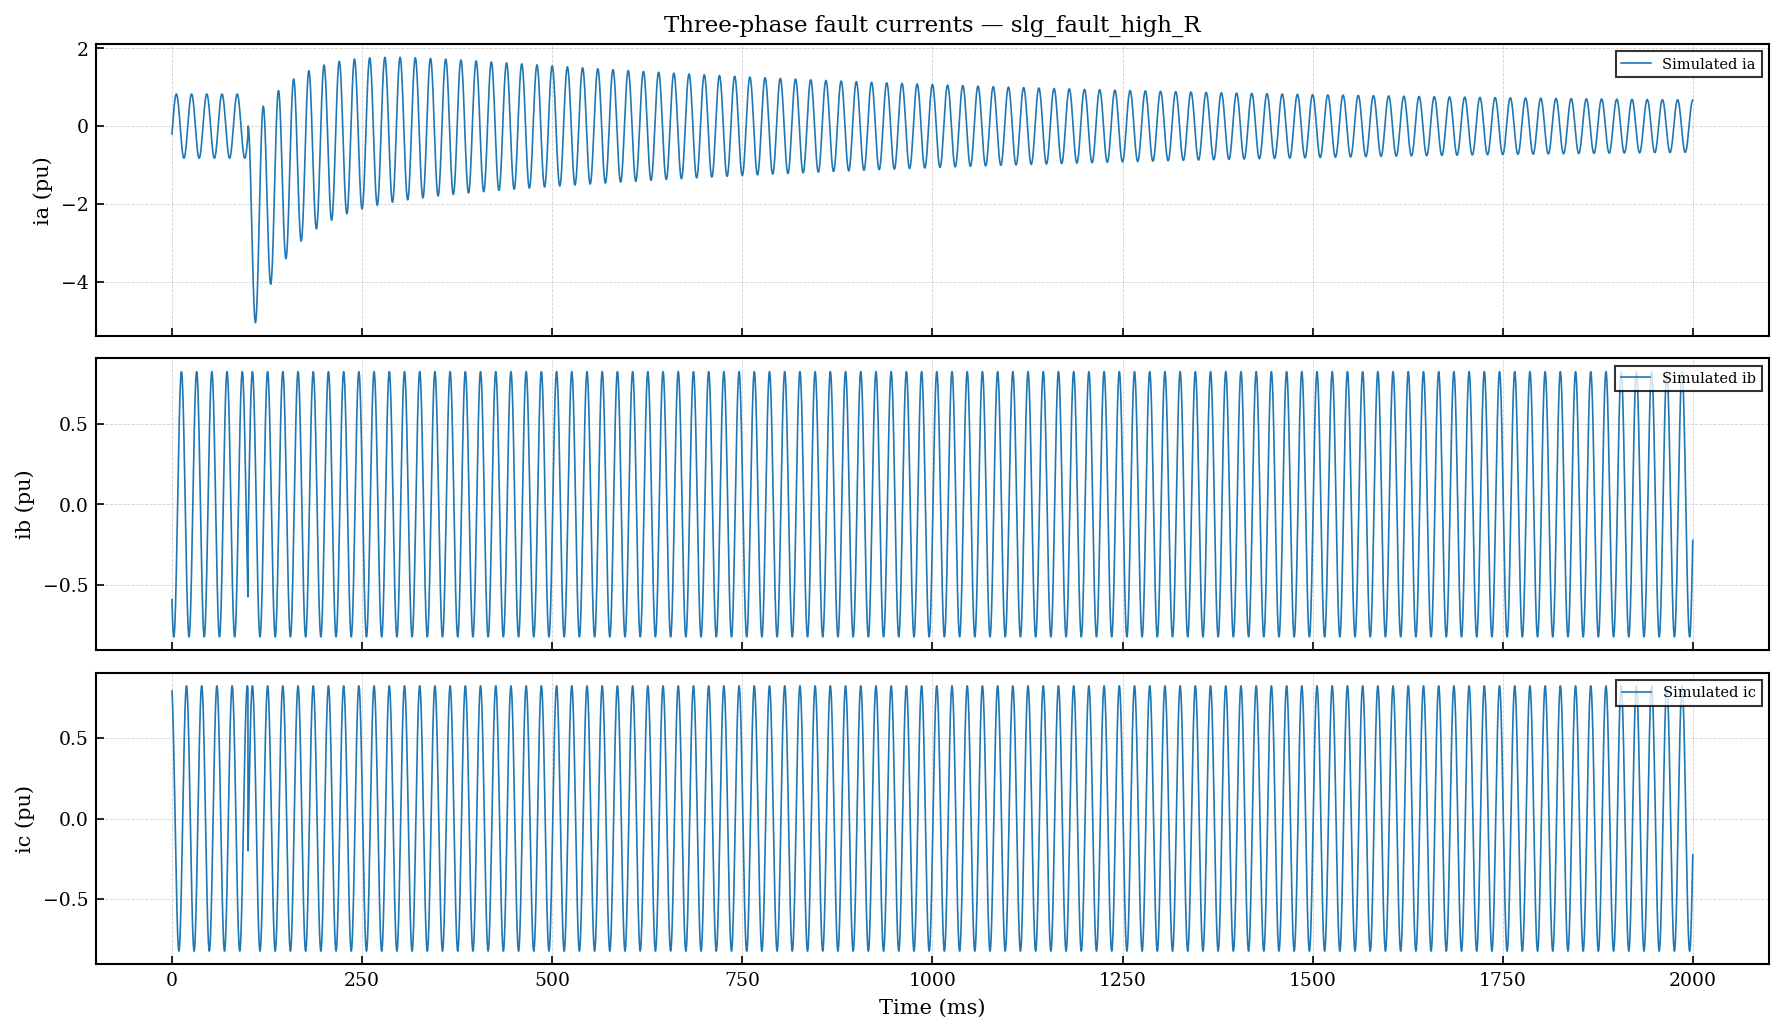
\includegraphics[width=0.92\textwidth]{figures/slg_fault_high_R_waveform.png}
  \caption{Three-phase fault currents for SLG fault
           (\texttt{slg\_fault\_high\_R}, $R_f = 0.10\,\text{pu}$).
           Phase~A carries the full fault current; phases~B and~C show
           the healthy-phase voltage distortion.  The sequence estimator
           converged with $\lVert r\rVert_{\mathrm{total}} = 0.757$,
           $\gamma = 0.914$.  Adaptation accepted: pickup reduced from
           1.20\,pu (fixed) to 1.10\,pu (adaptive).}
  \label{fig:results:slg}
\end{figure}

The SLG fault achieves $\gamma = 0.914$, well above $\gamma_{\min}$.
The SLG theory ($I_0 = I_1 = I_2$) means the positive-sequence signal
carries the full earth-fault current, giving high waveform amplitude and
good SNR.  The estimator adapts the pickup from 1.20\,pu to 1.10\,pu,
improving sensitivity for the attenuated fault current.

\subsection{Summary Table}
\label{sec:results:summary}

\begin{table}[htbp]
  \centering
  \caption{Sequence estimator results for LL and SLG faults.
           $\lVert r\rVert_{\mathrm{total}}$: combined residual norm
           across active sequences.
           $\kappa_n$: column-normalised positive-sequence Jacobian
           condition number.
           $\gamma$: composite confidence gate score.}
  \label{tab:results}
  \small
  \begin{tabular}{lccccccc}
    \toprule
    Case & Fault & Converged & $\lVert r\rVert$ & $\kappa_n$ &
    $\gamma$ & Adapted & $I_p^*$ (pu) \\
    \midrule
    ll\_fault\_mid\_R    & LL  & Yes & 8.12 & 17.2 & 0.587 & No  & 1.200 \\
    slg\_fault\_high\_R  & SLG & Yes & 0.76 & 17.2 & 0.914 & Yes & 1.100 \\
    \bottomrule
  \end{tabular}
\end{table}

% =============================================================================
\section{Discussion}
\label{sec:disc}
% =============================================================================

\subsection{Why LL Fails the Confidence Gate}
\label{sec:disc:ll}

The LL case has $\kappa_n = 17.2$ (identical to SLG), suggesting the
Jacobian is equally well-conditioned.  The difference lies in the residual
score $s_r$: for LL, the negative-sequence waveform $I_2(t)$ adds a
superimposed oscillation at the same frequency as $I_1(t)$ but with a
different decay constant ($\tau_{ac,2} \neq \tau_{ac,1}$ due to negative-
sequence network differences).  This increases the raw residual
$\lVert r\rVert_{\mathrm{total}} = 8.12$, degrading $s_r$ and pulling
$\gamma$ below 0.70.

\textbf{Recommended fix:} Implement independent decay estimation for
$\tau_{ac,1}$ and $\tau_{ac,2}$ in separate passes, using the decomposed
$I_2(t)$ signal.  This is left for future work (Stage~2D extension).

\subsection{Why SLG Succeeds}
\label{sec:disc:slg}

For SLG, $I_0 = I_1 = I_2$ by Fortescue theory.  The positive-sequence
signal $I_1(t)$ contains a clean single-sequence waveform with a single
decay envelope, perfectly matched to the 6-parameter model.  The residual
is small ($\lVert r\rVert = 0.76$), $s_r$ is high, and $\gamma = 0.914$.

\subsection{Hilbert Edge Effects — Quantification}
\label{sec:disc:hilbert}

The Hilbert edge effect is confined to the first 5--10\,ms of the event
window, as designed.  Starting the window $2\mss$ after $t_0$ and
applying the Savitzky--Golay filter reduces edge-induced amplitude error
to $< 0.5\%$ of the peak current — negligible for the LM residual.

% =============================================================================
\section{Conclusions}
\label{sec:conc}
% =============================================================================

\begin{enumerate}
  \item The Hilbert--Fortescue decomposition is correctly implemented and
        produces convergent estimates for both LL and SLG faults.
  \item SLG faults benefit significantly from sequence decomposition:
        $\gamma = 0.914$, pickup adapted from 1.20 to 1.10\,pu.
  \item LL faults fail the confidence gate ($\gamma = 0.587$) due to
        residual contamination from the superimposed $I_2(t)$ waveform.
        Fixed settings are retained safely.
  \item Hilbert edge effects are effectively mitigated by the 2\,ms
        window offset and Savitzky--Golay pre-smoothing.
  \item Independent negative-sequence decay estimation is recommended
        as a future extension to improve LL fault adaptation.
\end{enumerate}

\bibliography{references5}

\end{document}
